\documentclass[usenames,dvipsnames,tikz]{standalone}
%\usetikzlibrary{shapes.geometric}
%\usepackage{xcolor}
%\usepackage{tikz}
%\usepackage{standalone}
\usepackage{amsmath}
\usepackage{mathtools}

%Tikz colours, used in tikz figures only
\colorlet{tBlue}{RoyalBlue!35!Cerulean} %tikz color
\colorlet{tRed}{Red} %tikz color
\definecolor{tGreen}{HTML}{569909} %tikz color
\definecolor{tOrange}{HTML}{FA7602} %tikz color
\definecolor{tLightGreen1}{HTML}{C1E685} %tikz color
\definecolor{tLightOrange1}{HTML}{FFCD4F} %tikz color
\colorlet{tLightGreen}{LimeGreen!70!OliveGreen!45!White}
\colorlet{tLightOrange}{Dandelion!65!White}
\definecolor{tLightPink}{HTML}{FFD4EB} %tikz color
\definecolor{tLightBlue}{HTML}{CEF0FF} %tikz color

%Text colours
\colorlet{myRed}{Red!50!OrangeRed}
\definecolor{myOrange}{HTML}{FA7602}
\definecolor{myGreen}{HTML}{569909}
\definecolor{myAqua}{HTML}{00B1BA} %02BEB8
\definecolor{myBlue}{HTML}{0095FF} %00B3FF
\colorlet{myPurple}{Orchid} 
\colorlet{myPink}{Rhodamine!65!Lavender}
\colorlet{myGray}{Gray!90!White}
\begin{document}	
	
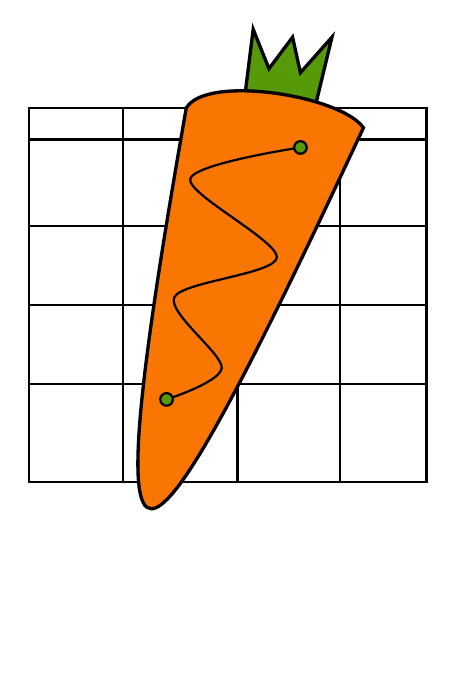
\begin{tikzpicture}
%\draw [help lines] (-1,-1) grid (10, 10);



%----------------------------------------------------------------
% R1
%\node at (3,5.3) {\small{$R^*_1$}};
%\draw (2.95,5.6) -- (2.95, 5.2) -- (2.85,5.2) -- (3,5) -- (3.15,5.2) -- (3.05,5.2) -- (3.05,5.6) -- (2.95,5.6);

%\draw [thick, tRed] (2,2.75) -- (2,3.75);
%\draw [thick, tRed] (3,2.75) -- (3,3.75);
%\draw [thick, tRed] (4,2.75) -- (4,3.75);

%\draw [thick, densely dashed, tGreen] (2,3.75) -- (3,2.75);
%\draw [thick, densely dashed, tGreen] (3,3.75) -- (4,2.75);
%\draw [thick] (3.25,6) to [out=260,in=245, distance=7cm] (5.5,5.75);
%\draw [thick] (3.25,6) to[out=60,in=125, distance=0.5cm] (5.5,5.75);



%\draw [thick] (4.25,6.2) to[out=120,in=240] (4.25,7);

\draw [thick] (1.25,6) rectangle (6.3,1.25);
\draw [thick] (1.25, 5.6) -- (6.3, 5.6);
\draw [thick] (1.25, 4.5) -- (6.3, 4.5);
\draw [thick] (1.25, 3.5) -- (6.3, 3.5);
\draw [thick] (1.25, 2.5) -- (6.3, 2.5);

\draw [thick] (2.45, 6) -- (2.45, 1.25);
\draw [thick] (3.9,6) -- (3.9, 1.25);
\draw [thick] (5.2, 6) -- (5.2, 1.25);

\draw [very thick, fill=tGreen] (4,6.2) -- (4.1,7) -- (4.3, 6.5) -- (4.6, 6.9) -- (4.7, 6.45) -- (5.1, 6.9) -- (4.9, 6.07) -- (4,6.2);

\draw [very thick, fill=tOrange] (3.25,6) to[out=260,in=245, distance=7cm] (5.5,5.75) to[out=125,in=60, distance=0.5cm] (3.25,6);

%\draw [thick] (2.9, 1.5) to[out=350, in=30] (3.1, 2.6);

%\draw [thick] plot [smooth] coordinates { (2.9,2.3) (3.7,2.6) (3,3.4) (4.2, 3.7) (3.2, 4.6) (4.4, 4.8)};
\draw [thick] plot [smooth] coordinates { (3,2.3) (3.7,2.7) (3.1,3.6) (4.4, 4.1) (3.3, 5.1) (4.7, 5.5)};

\draw [thick, fill=tGreen] (3,2.3) circle [radius = 0.08];
\draw [thick, fill=tGreen] (4.7,5.5) circle [radius = 0.08];



%\draw [thick] (4.25,6.2) to[out=50,in=320] (3.75,7.25);
%\draw [thick] (4.25,6.2) to[out=50,in=320] (3.75,7.25);

%\draw [fill=white, thick] (2,2.75) circle [radius = 0.08];
%\draw [fill=white, thick] (3,2.75) circle [radius = 0.08];
%\draw [fill=white, thick] (4,2.75) circle [radius = 0.08];
%\draw [fill=white, thick] (2,3.75) circle [radius = 0.08];
%\draw [fill=white, thick] (3,3.75) circle [radius = 0.08];
%\draw [fill=white, thick] (4,3.75) circle [radius = 0.08];

%\node at (2,2.45) {\large{$v_{17}$}};
%\node at (3,2.45) {\large{$v_{16}$}};
%\node at (4,2.45) {\large{$v_{15}$}};
%\node at (2,4.05) {\large{$v_2$}};
%\node at (3,4.05) {\large{$v_3$}};
%\node at (4,4.05) {\large{$v_4$}};


%-------------------------------------------
% R2
%\node at (7.5,5.3) {\small{$R^*_2$}};
%\draw (7.45,5.6) -- (7.45, 5.2) -- (7.35,5.2) -- (7.5,5) -- (7.65,5.2) -- (7.55,5.2) -- (7.55,5.6) -- (7.45,5.6);

%\draw [thick, tRed] (7,2.75) -- (7,3.75);
%\draw [thick, tRed] (8,2.75) -- (8,3.75);

%\draw [very thick, dotted, tOrange] (7,3.75) -- (8,2.75);
%\draw [very thick, dotted, tOrange] (8,3.75) to[out=120,in=140, distance=2cm] (7,2.75);

%\draw [fill=white, thick] (7,2.75) circle [radius = 0.08];
%\draw [fill=white, thick] (8,2.75) circle [radius = 0.08];
%\draw [fill=white, thick] (7,3.75) circle [radius = 0.08];
%\draw [fill=white, thick] (8,3.75) circle [radius = 0.08];

%\node at (7,2.45) {\large{$v_{12}$}};
%\node at (8,2.45) {\large{$v_{11}$}};
%\node at (7,4.05) {\large{$v_7$}};
%\node at (8,4.05) {\large{$v_8$}};

%--------------------------------------
%New set of edges R'
%\draw [thick, tRed] (1,0) -- (1,1);
%\draw [thick, densely dashed, tGreen] (2,0) -- (2,1);
%\draw [thick, densely dashed, tGreen] (3,0) -- (3,1);
%\draw [thick, densely dashed, tGreen] (4,0) -- (4,1);
%\draw [thick, tRed] (5,0) -- (5,1);
%\draw [thick, tRed] (6,0) -- (6,1);
%\draw [very thick, dotted, tOrange] (7,0) -- (7,1);
%\draw [very thick, dotted, tOrange] (8,0) -- (8,1);
%\draw [thick, tRed] (9,0) -- (9,1);
%
%\draw [fill=white, thick] (1,0) circle [radius = 0.08];
%\draw [fill=white, thick] (2,0) circle [radius = 0.08];
%\draw [fill=white, thick] (3,0) circle [radius = 0.08];
%\draw [fill=white, thick] (4,0) circle [radius = 0.08];
%\draw [fill=white, thick] (5,0) circle [radius = 0.08];
%\draw [fill=white, thick] (6,0) circle [radius = 0.08];
%\draw [fill=white, thick] (7,0) circle [radius = 0.08];
%\draw [fill=white, thick] (8,0) circle [radius = 0.08];
%\draw [fill=white, thick] (9,0) circle [radius = 0.08];
%
%\draw [fill=white, thick] (1,1) circle [radius = 0.08];
%\draw [fill=white, thick] (2,1) circle [radius = 0.08];
%\draw [fill=white, thick] (3,1) circle [radius = 0.08];
%\draw [fill=white, thick] (4,1) circle [radius = 0.08];
%\draw [fill=white, thick] (5,1) circle [radius = 0.08];
%\draw [fill=white, thick] (6,1) circle [radius = 0.08];
%\draw [fill=white, thick] (7,1) circle [radius = 0.08];
%\draw [fill=white, thick] (8,1) circle [radius = 0.08];
%\draw [fill=white, thick] (9,1) circle [radius = 0.08];
%
%\node at (1,-0.3) {\large{$v_{18}$}};
%\node at (2,-0.3) {\large{$v_{16}$}};
%\node at (3,-0.3) {\large{$v_{15}$}};
%\node at (4,-0.3) {\large{$v_{17}$}};
%\node at (5,-0.3) {\large{$v_{14}$}};
%\node at (6,-0.3) {\large{$v_{13}$}};
%\node at (7,-0.3) {\large{$v_{11}$}};
%\node at (8,-0.3) {\large{$v_{12}$}};
%\node at (9,-0.3) {\large{$v_{10}$}};
%
%\node at (1,1.3) {\large{$v_1$}};
%\node at (2,1.3) {\large{$v_2$}};
%\node at (3,1.3) {\large{$v_3$}};
%\node at (4,1.3) {\large{$v_4$}};
%\node at (5,1.3) {\large{$v_5$}};
%\node at (6,1.3) {\large{$v_6$}};
%\node at (7,1.3) {\large{$v_7$}};
%\node at (8,1.3) {\large{$v_8$}};
%\node at (9,1.3) {\large{$v_9$}};




\end{tikzpicture}
	
\end{document}